\documentclass[../main.tex]{subfiles}
\begin{document}
\chapter{Particle identification and reconstruction}
\label{intro:sec:id}

Each type of particle resulting from the $pp$ collision, its decay products or the outcome of its hadronization, leaves a signature in the detector, as shown in Fig.~\ref{intro:fig:cms_slice}. Muons lose an small fraction of its energy in the inner part of the detector, so, as they are charged particles, are detected in both the inner tracker and the muon chambers. Electrons and photons are both absorbed in the ECAL (where their energy can be measured), although only the electrons leave a track in the inner tracker. Hadrons cross the ECAL with low energy loss, depositing most of their energy in the HCAL. The trajectory of the charged hadrons can be measured in the tracker. Neutrinos hardly interact with the CMS detector and they escape it. However, they manifest their presence by the energy imbalance of the event in the transverse plane or missing transverse energy.

\begin{figure}[h!]
\begin{center}

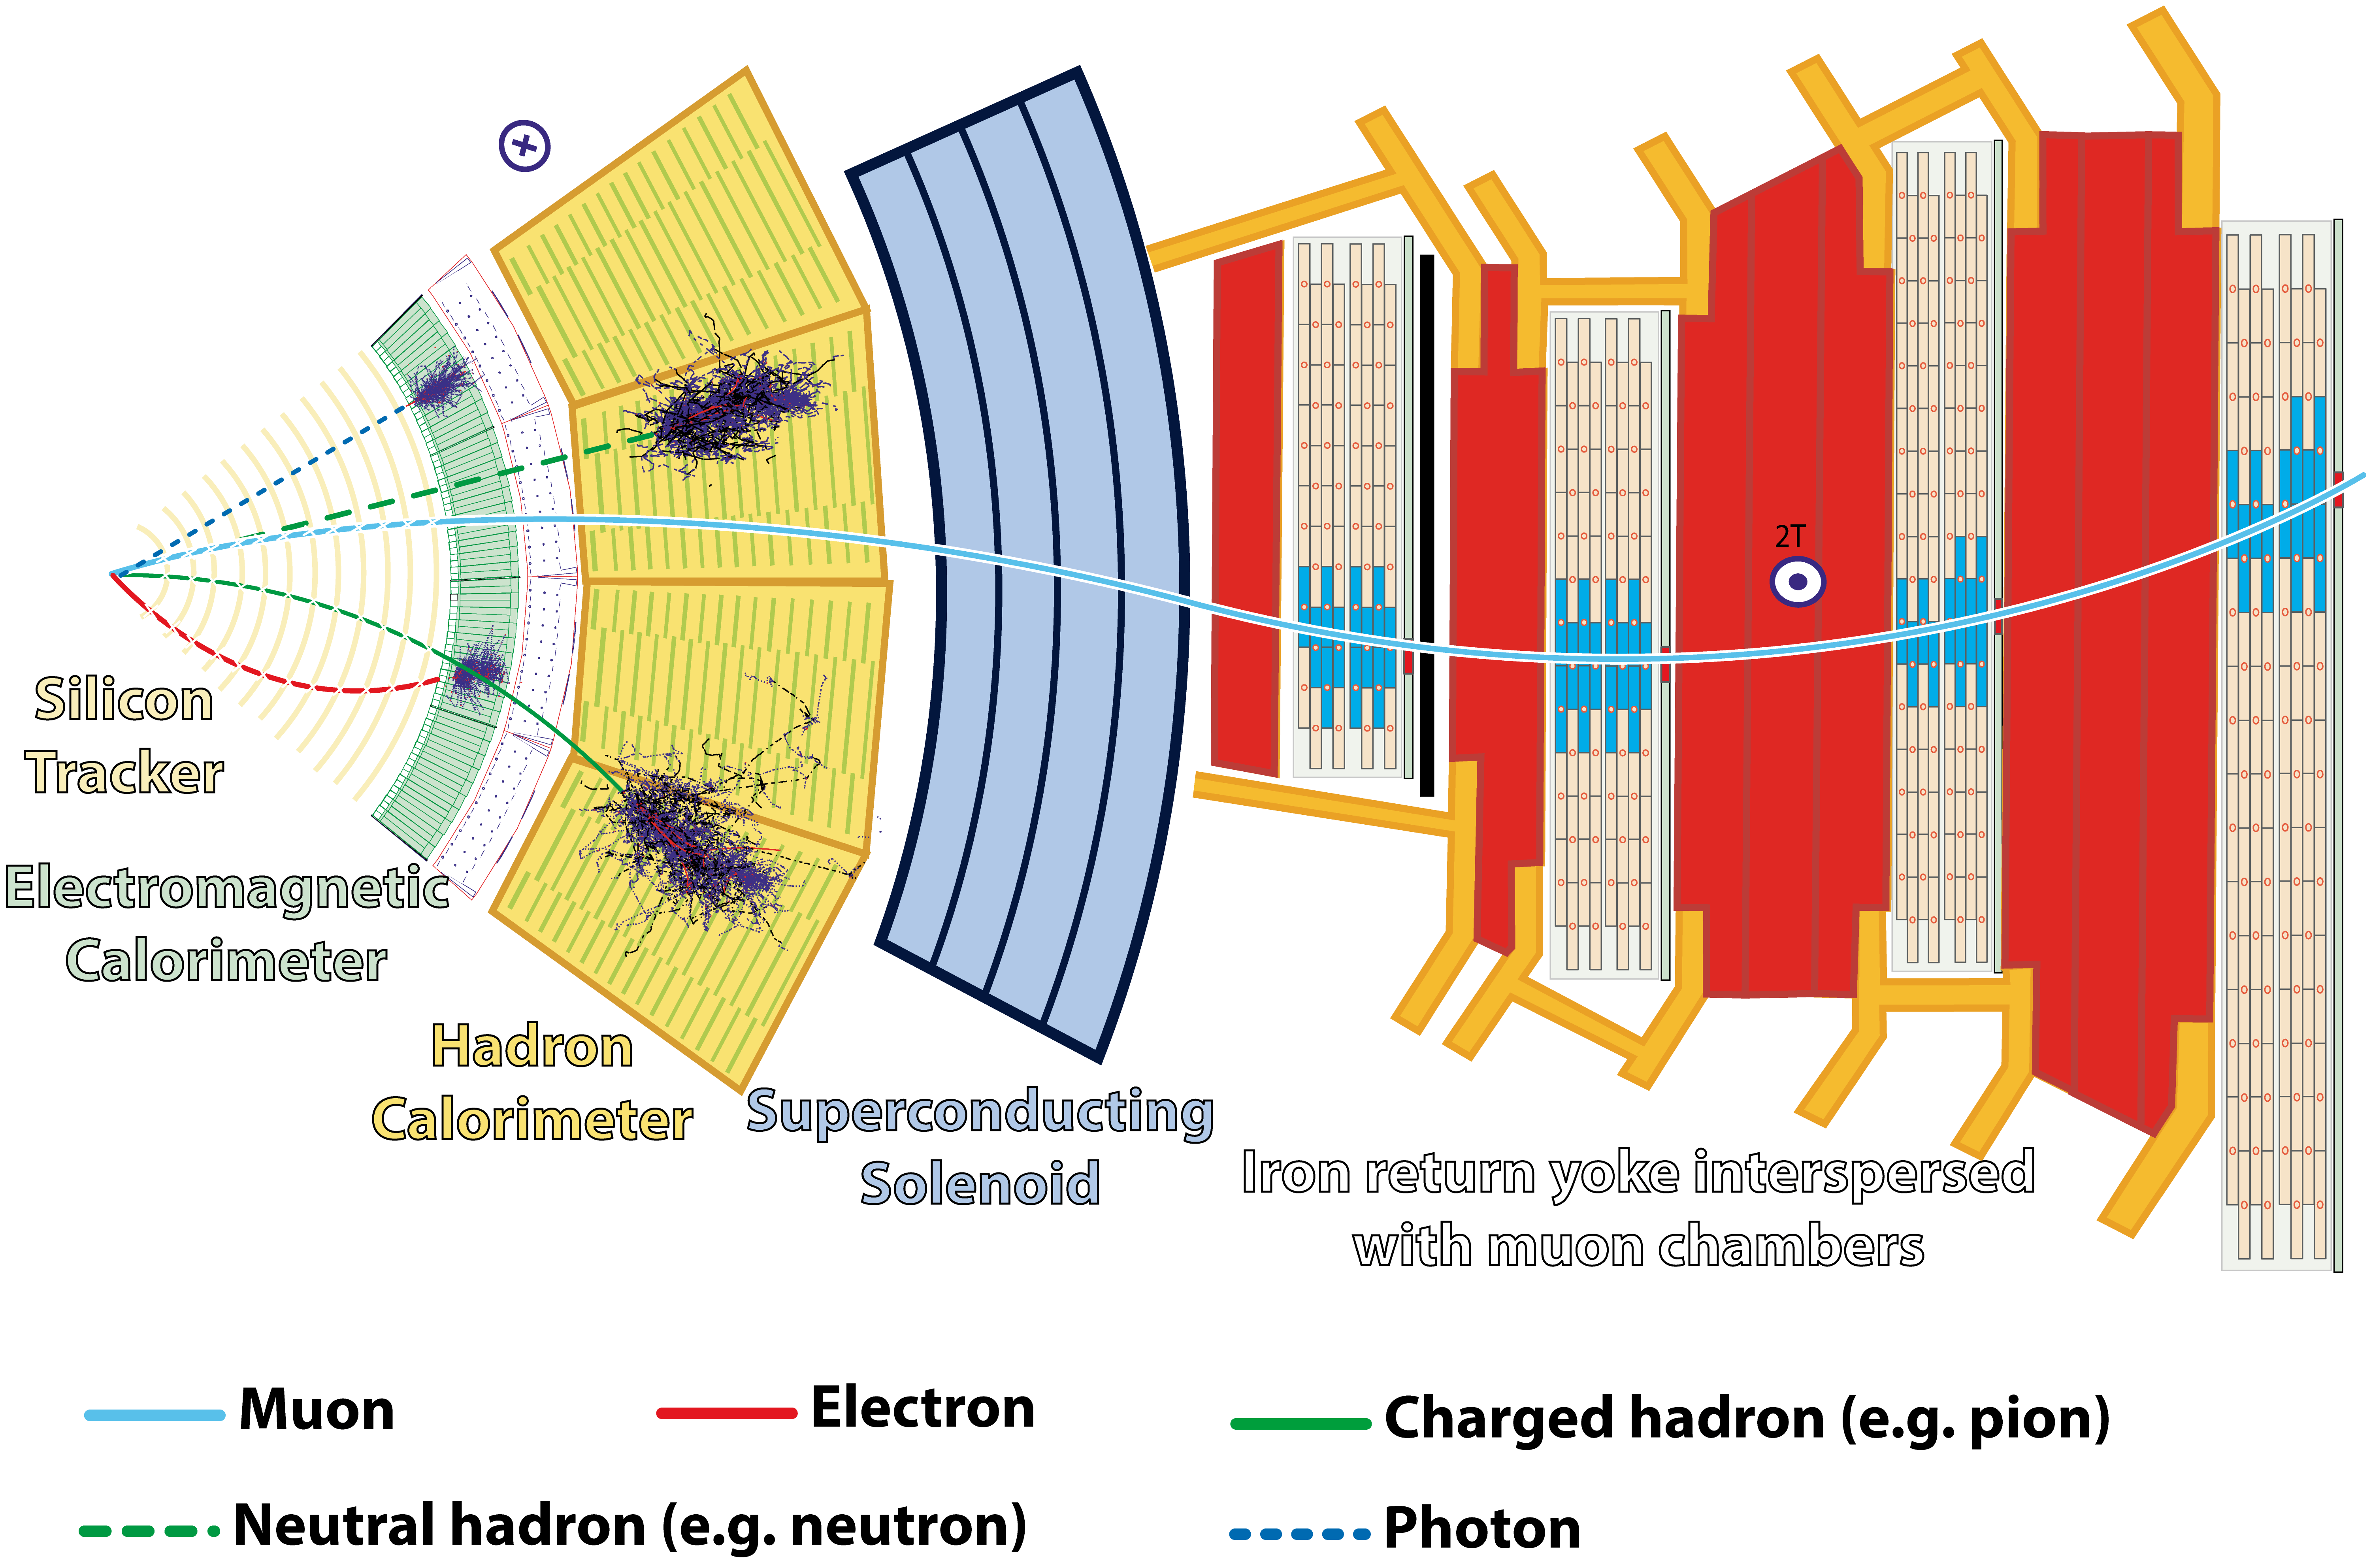
\includegraphics[width=0.7\textwidth]{Images/CMSslice_whiteBackground}
\end{center}
\caption{Slice of the CMS detector in the transverse view with the signals left by different particles. Extracted from \cite{hh:intro:cms_slice}.}
\label{intro:fig:cms_slice}
\end{figure}

In order to reconstruct the physics objects, the information coming from all subdetectors is combined by the Particle Flow (PF) \cite{intro:id:pf}  algorithm. This algorithms attempts a correlation of basic elements from all the detector layers to identify each final-state particle (with its energy and direction) and their possible combinations in order to build higher level objects, such as tau leptons or jets.

\section{The Particle Flow algorithm}

\textcolor{red}{TODO.}

\section{Final state particle reconstruction}

\subsection{Muons}
\label{intro:subsec:muon}

Muons are reconstructed independently by the silicon tracker and the muon chambers \cite{intro:id:muon_7tev}. The former gives a precise measurement of the momentum of these muons, while the latter identifies muons with high efficiency over the full detector acceptance. Muon objects are reconstructed as three different muon types:
\begin{itemize}
\item Hits coming from the DT and CSC systems are identified and clustered in ordered to build straight-line track \textit{segments}. This is also known as \textit{local} reconstruction. Then, local segments and hits coming from the DT, CSC and RPC can be combined into \textbf{standalone muons}.
\item Standalone muon tracks can be matched to tracks in the inner tracker and, if they are compatible when propagated onto a common surface, a \textbf{global muon} is constructed.
\item Tracks reconstructed in the inner tracker can be extrapolated to the muon system. If at least one muon segment matches the extrapolation, the track is identified as a \textbf{tracker muon} track.
\end{itemize}

Thanks to the high efficiency of the inner track and muon segment reconstruction, about 99\% of the muons produced with the geometrical acceptance of the muon system are reconstructed as global or tracker muons, and very often as both. If this is the case, they are merged into a single candidate.

Charged hadrons may be misreconstructed as muons if, for example, some of the hadron shower remnants reach the muon system (\textit{punch-through}). This is taken into account by the PF algorithm in order to build PF muons by selecting some properties from global and tracker muons. Different levels of requirements (e.g. track fit $\chi^2$, number of hits per track or degree of matching between tracker and standalone tracks) result in three muon identification working points, \textit{loose}, \textit{medium} and \textit{tight}, with increasing purity and decreasing efficiency. The information from the different subdetectors is used to define the PF muon isolation:
\begin{equation}
	I_{rel}^l = \left(\sum p_T^{\text{charged}} + \max \left[ 0, \sum p_T^{\text{neutral-had}}  + \sum p_T^\gamma - \frac{1}{2}\sum p_T^{\text{PU}}	
	 \right] \right) / p_T^l,
\label{id:eq:iso}
\end{equation}
where $\sum p_T^{\text{charged}}$, $\sum p_T^{\text{neutral-had}}$, $\sum p_T^\gamma$, and $\sum p_T^{\text{PU}}$ are the scalar sums of the transverse momenta of charged hadrons originating from the primary vertex, neutral hadrons, photons, and charged hadrons not originating from the primary vertex respectively inside a $\Delta R < 0.4$ cone around the muon.

\subsection{Electrons}
\label{intro:subsec:ele}

Electrons are reconstructed using the information from the tracker and the ECAL \cite{intro:id:ele}. Because of the material of the tracker, most electrons emit a sizeable fraction of their energy as bremsstrahlung photons before entering the ECAL, so several ECAL clusters are produced. The energy of the electron and all possible produced photons is collected by grouping compatible clusters in a small window in $\eta$ and an extended window in $\phi$ (to account for the magnetic field) around the electron direction into \textit{superclusters}. Electron tracks are then reconstructed from the superclusters and tracker tracks refitted using a Gaussian-Sum Filter algorithm \cite{intro:id:gsf}.

Several strategies are used in order to discriminate prompt electrons from background sources. Electron PF isolation is computed using \eqref{id:eq:iso}, although the cone around the electron is defined with a $\Delta R < 0.3$. Three isolation components are considered separately, the scalar sums of transverse momenta of charged hadrons coming from the primary vertex, neutral hadrons and photons.

Electron identification is performed with a multivariate approach (MVA) updated and improved for Run 2 analysis \cite{intro:id:ele_mva}. The discriminator used is based on a Boosted Decision Tree (BDT) that considers as input variables related to the shower shape, the track quality, the track-cluster matching or the fraction of momentum lost due to brehmsstrahlung. To increase the flexibility at analysis level, two different BDTs are trained, one with the previous input variables and another one with those variables and the three isolation components as input. Several trainings are performed in bins of $E_T$ and $\eta$. The split in $E_T$ is at 10 GeV, so two regions where the background compositions are very different are defined. Two splits are defined in $\eta$: at $|\eta|<0.8$, where the tracker material budget starts to steeply increase, and in the barrel-endcap transition. Fig.~\ref{intro:fig:ele_mva} shows the performance of the BDTs for electrons with $E_T > 20$ GeV in the barrel and the endcap. Three working points are defined for the two BDTs (with and without the isolation variables): \textit{wp90} and \textit{wp80}, associated to a 90 and 80\% signal efficiency respectively, and a \textit{loose} WP, with 98\% signal efficiency.

\begin{figure}[h!]
\begin{center}
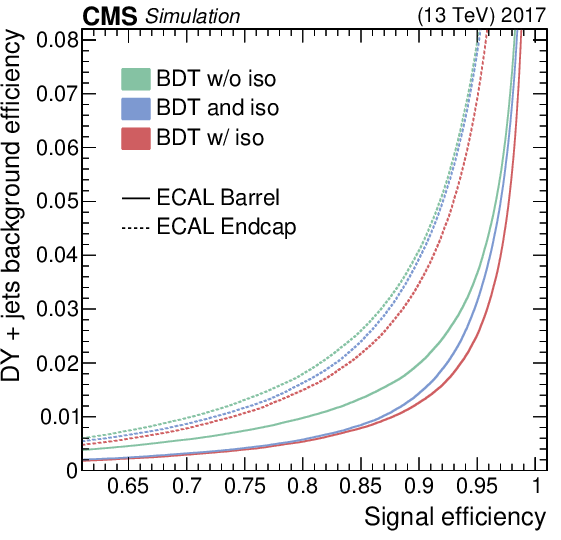
\includegraphics[width=0.6\textwidth]{Images/ele_mva}
\end{center}
\caption{Performance of the electron MVA-based identification algorithm with (red) and without (green) the isolation variables, compared to an optimized sequential selection using the BDT without the isolations followed by a selection requirement on the combined isolation (blue). Electrons are selected for the training with an $E_T$ of at least 20 GeV. Extracted from \cite{intro:id:ele_mva}.}
\label{intro:fig:ele_mva}
\end{figure}


\subsection{Jets}
\label{intro:subsec:jets}

Jets are originated by the hadronic showers produced from quarks and gluons. In the experiment, they can be reconstructed by clustering charged and neutral hadrons with the anti-$k_T$ algorithm \cite{intro:id:antikt}. This clustering is done by grouping PF candidates close to each other in order to build a cone-shaped jet whose size is determined by the distance parameter $R$. Regular jets, or AK4 jets, are reconstructed with a distance parameter of 0.4. In boosted topologies, where the particle decaying into two jets has very high momentum, both AK4 jets can overlap. Therefore, a bigger object with distance parameter $R=0.8$ can be built, corresponding to an AK8 jet. 

To reduce jets poorly reconstructed or affected by instrumental noise in the calorimeters, some identifications requirements are applied to them \cite{intro:id:pfjetid}. Some of these requirements are the fraction of charged and neutral hadrons, electrons, photons and muons or the multiplicity of charged and neutral hadrons. Three working points are considered, \textit{loose} and \textit{tight} (designed to remove jets originating from calorimetric noise) and \textit{tight lepton veto}, that rejects background coming from mis-reconstructed electron and muon candidates. The performance of the tight working point is shown in Fig.~\ref{intro:fig:jetid}.

\begin{figure}[h!]
\begin{center}
\subfloat{\includegraphics[width=0.45\textwidth]{Images/Figure_003-a}}
\subfloat{\includegraphics[width=0.45\textwidth]{Images/Figure_003-b}}\\
\subfloat{\includegraphics[width=0.45\textwidth]{Images/Figure_004-a}}
\subfloat{\includegraphics[width=0.45\textwidth]{Images/Figure_004-b}}
\end{center}
\caption{Performance of the CMS PF jet identification algorithm for the tight working point. Plots from the top row show the efficiency of correctly identifying a PF jet, while the ones in the bottom row show the noise jet background rejection rate. The two plots from the left are shown as a function of the jet $p_T$ for central jets ($|\eta|<0.5$), while right plots are shown as a function of the jet $|\eta|$ for jets with $p_t$ between 30 and 100 GeV. Extracted from \cite{intro:id:pfjetid}.}
\label{intro:fig:jetid}
\end{figure}

PU jets are jets not coming from the primary vertex, so they do not come from the interaction under study. To reduce the amount of them, several mitigation techniques exist to identify and reject such jets \cite{intro:id:pujet}. The most commonly used is the Charged Hadron Substraction (CHS), which removes all charged constituents associated to secondary vertices before starting the jet clustering procedure. After applying the CHS mitigation technique, the remaining PU jets are further reduced by applying a multivariate approach, the PU jet ID. It consists of a BDT trained with 12-15 variables that characterize the jet and the event. The performance of this algorithm is shown in Fig.~\ref{intro:fig:pujetid}.  Three working points are defined for this discriminant, the \textit{tight} and medium working points, with 80 and 90\% efficiency on quark jets respectively, and the loose working point, 99\% efficient for quark jets in $|\eta|<2.5$ and 95\% efficient for quark jets in $|\eta|>2.5$.


\begin{figure}[h!]
\begin{center}
\subfloat{\includegraphics[width=0.6\textwidth]{Images/ROC_PUID_eta0to2p5}}
\end{center}
\caption{PU Jet ID mistag rate as a function of its efficiency for jets with $|\eta|<2.5$ and $p_T\in[20, 50]$ GeV. Performance is measured by using simulated samples of Drell-Yan events. Extracted from \cite{intro:id:pujetid}}
\label{intro:fig:pujetid}
\end{figure}


In order to identify jets coming from the hadronisation of b quarks (b-jets), dedicated algorithms have been developed. Among those we can find the DeepCSV \cite{intro:id:deepcsv} and DeepJet \cite{intro:id:deepflavour} algorithms. Both algorithms are DNN-based approaches, although the latter shows a better performance (shown in Fig.~\ref{intro:fig:btag}) thanks to including the full information of all jet constituents, neutral and charged particles, secondary vertices and global event variables. Three working points are defined, \textit{loose}, \textit{medium} and \textit{tight}, corresponding to around 10, 1 and 0.1~\% light jet misidentification probability respectively.

\begin{figure}[h!]
\begin{center}
\includegraphics[width=0.6\textwidth]{Images/btag}
\end{center}
\caption{Performance of the CMS DeepJet (blue) and DeepCSV (red) algorithms.  
The plot represents the probability of misidentifying jets coming from light quarks or gluons (solid lines) or c jets (dashed lines) with respect to the efficiency of correctly identifying jets coming from b quarks. Results are obtained using jets with $|\eta|<2.5$ and $p_T>30$~GeV coming from the decay of simulated $\text{t}\bar{\text{t}}$ events. Loose, medium and tight working points for both algorithms are shown in the plot as circles when obtained directly from the simulation or as triangles after applying the scale factors obtained through data-simulation studies. Extracted from \cite{intro:id:deep_csv_jet}.}
\label{intro:fig:btag}
\end{figure}

\subsection{Tau leptons}
\label{intro:subsec:taus}

The $\tau$ lepton is the heaviest lepton, with a mass of $m_\tau = 1.777~$ GeV. This mass is enough to make it decay immediately after its production into a lighter lepton and two neutrinos (leptonic decay) or into hadrons and a $\tau$ neutrino (hadronic decay). In the leptonic decays, the $\tau$ is reconstructed as the correspondent electron or muon. In the hadronic decays, however, the $\tau$ lepton usually decays to charged hadrons (mostly $\pi^\pm$), denoted as \textit{prongs}, and neutral hadrons ($\pi_0$). Therefore, the hadronic $\tau$ ($\tau_h$) has to be reconstructed as a composite object from its PF components. In both decays, neutrinos remain undetected, so it's not possible to measure exactly the momentum of the decaying $\tau$. A summary of the existing $\tau$ decay modes and their branching fractions in shown in Table~\ref{id:tab:tau_decay}.


\begin{table}
\begin{center}
\begin{tabular}{l  r}
Decay Mode & BR (\%)\\\hline\hline
Leptonic decays \\
$\tau^- \to e^-\bar{\nu}_e\nu_\tau$ & 17.8 \\
$\tau^- \to \mu^-\bar{\nu}_\mu\nu_\tau$ & 17.4 \\\hline
Hadronic decays \\
$\tau^- \to$~h${}^-\nu_\tau$ & 11.5 \\
$\tau^- \to$~h${}^-\pi^0\nu_\tau$ & 25.9 \\
$\tau^- \to$~h${}^-\pi^0\pi^0\nu_\tau$ & 9.5 \\
$\tau^- \to$~h${}^-$h${}^+$h${}^-\nu_\tau$ & 9.8 \\
$\tau^- \to$~h${}^-$h${}^+$h${}^-\pi^0\nu_\tau$ & 4.8 \\
Other & 3.3
\end{tabular}
\end{center}
\caption{Decay modes of the $\tau$ lepton and their branching fractions (BR) in \% \cite{pdg}. Charged hadrons are denoted by h${}^\pm$.}
\label{id:tab:tau_decay}
\end{table}


For the $\tau_h$ reconstruction, the \textit{hadrons-plus-strips} (HPS) algorithm \cite{intro:id:hps} is used. This algorithm is seeded by the AK4 PF jets reconstructed as in Section~\ref{intro:subsec:jets} and its constituents. Regarding the $\pi_0$, they promptly decay into a pair of photons, which can then convert into $e^+e^-$ pairs thanks to the amount of tracker material. Electrons and photon candidates in a certain region $\Delta\phi\times\Delta\eta$ are clustered together, building \textit{strips}, so the energy of the $\pi_0$ is measured. Both charged hadrons and strips inside the PF jet are then combined by the HPS algorithm into all the possible combinations of hadrons for the following decay modes: $\text{h}^\pm$, $\text{h}^\pm\pi^0$, $\text{h}^\pm\pi^0\pi^0$ and $\text{h}^\pm \text{h}^\mp \text{h}^\pm$ (plus the additional $\nu_\tau$).


In order to increase the purity of the $\tau_h$ reconstruction, an identification method, \deeptau{} \cite{intro:id:deeptau}, has been implemented to discriminate real $\tau_h$ from quark and gluon jets, electrons and muons. This algorithm follows a multi-class DNN approach that combines information from high-level reconstructed $\tau$ features, the decay mode extracted from the HPS algorithm and low-level information used to build the PF candidates. Three different discriminators, built to identify $\tau_h$ against jets, electrons and muons, respectively, are defined within the \deeptau{} algorithm, each with its own associated working points:
\begin{itemize}
	\item \textit{DeepTauVSjet}, with working points VVVLoose (very-very-very-loose), VVLoose, VLoose, Loose, Medium, Tight, VTight and VVTight.
	\item \textit{DeepTauVSe}, with working points VVVLoose, VVLoose, VLoose, Loose, Medium, Tight, VTight and VVTight.
	\item \textit{DeepTauVSmu}, with working points VLoose, Loose, Medium and Tight.
\end{itemize}
The performance of the three discriminators is shown in Fig.~\ref{intro:fig:deeptau}, where a substantial improvement with respect to older algorithms can be seen.


\begin{figure}[h!]
\begin{center}
\subfloat[DeepTauVSjet]{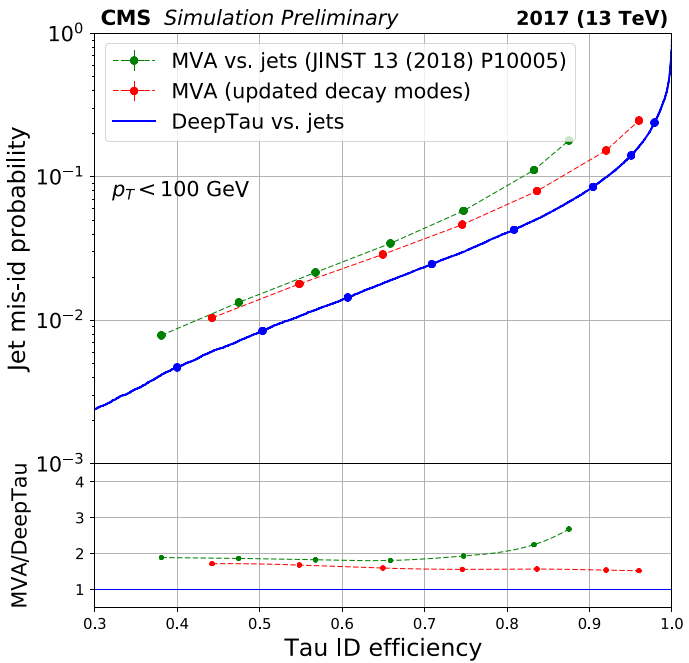
\includegraphics[width=0.45\textwidth]{Images/deeptauvsjet}}
\subfloat[DeepTauVSe]{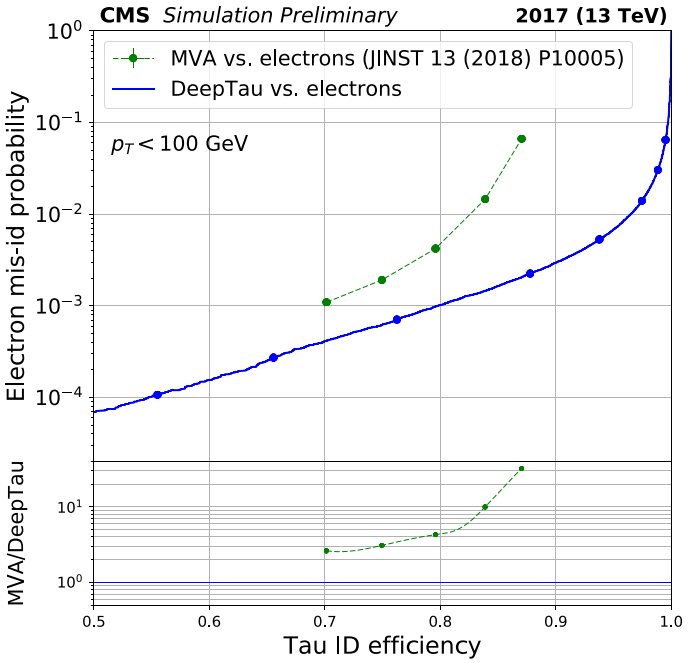
\includegraphics[width=0.45\textwidth]{Images/deeptauvse}} \\
\subfloat[DeepTauVSmu]{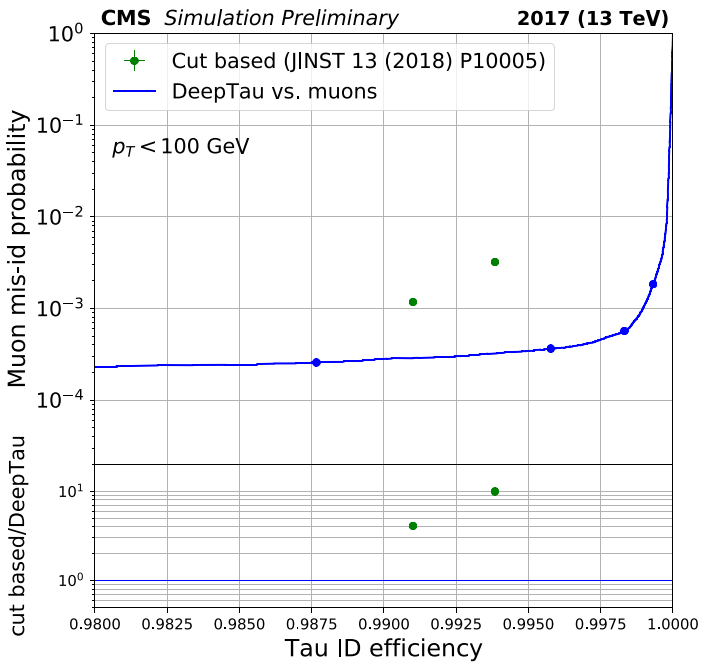
\includegraphics[width=0.45\textwidth]{Images/deeptauvsmu}}
\end{center}
\caption{Performance of the CMS \deeptau{} algorithm. Plots represent the probability of misidentify jets (a), electrons (b) or muons (c) as $\tau_h$ with respect to the efficiency of correctly identifying the $\tau_h$ for the DeepTauVSjet (a), DeepTauVse (b) and DeepTauVSmu (c) discriminators. Working points of the discriminators are indicated as dots. The performance of older discriminators used before the appearance of the \deeptau{} algorithm are also shown for the sake of comparison. Extracted from \cite{intro:id:deeptau}.}
\label{intro:fig:deeptau}
\end{figure}

\subsection{Missing transverse energy}
\label{intro:subsec:met}

When two protons collide, the amount of momentum carried by their constituents is unknown. However, their momentum in the transverse plane can be considered as negligible. Therefore, by conservation of momentum, the total momentum in the transverse plane in the initial and in the final state should also be negligible. Then, particles that can't be measured in the detector (neutrinos, BSM particles,...) can be observed by an energy imbalance in the transverse plane. The \textit{missing transverse momentum} is then defined as
\begin{equation}
	\vec{p}_T{}^{\text{miss}} = - \sum \vec{p}_T,
\end{equation}
where the sum extends to all the PF particles available in each event. The modulus of $\vec{p}_T{}^{\text{miss}}$ can be denoted as $p_T^{\text{miss}}$.

To perform a precise measurement of this quantity, the CMS detector should cover almost the whole solid angle, so most of the particles that can be measured go through the detector. But its determination is also affected by inefficiencies of tracking and clustering algorithms or from the actual detector (for example, calorimeter noise). Anomalous events that could have a large missing energy coming from detector issues are removed by using specific filters prior to any analysis \cite{intro:id:met}.


\end{document}

